% !TEX root = ../main.tex
\documentclass[../main.tex]{subfiles}

\begin{document}
\section{Secure Command Line Interface}

The command line interface of the application depends on communication via a Unix domain socket \cite{unix_domain_socket},
guaranteeing secure communication accessible only by having system access to the running application.
The location of the socket alogiside the feature toogle is defined by the application configuration file.

\subsection{Application config system}

The application configuration files are stored in YAML file format \cite{yaml}.
Configuration system is hierarchical, if files are stored in multiple locations they are merged together.
The config files can have either \textbf{.yml} or \textbf{.yaml} file extension.
Name of the file can be one of the following:
\begin{itemize}
  \item \textbf{hydra}
  \item \textbf{hydra-config}
  \item \textbf{hydra.config}
\end{itemize}

Additionally, each configuration file can have a \textbf{.local} added before the file extension, e.g. \textbf{hydra.local.yml}. This is reffered to as \textbf{local} configuration file.
Also, a dot can be added to the start of the file name, e.g. \textbf{.hydra.yml}. This is reffered to as \textbf{hidden} configuration file. Other configuration files are reffered to as \textbf{normal} or \textbf{standard} configuration files.

When configuration files are merged they are merged in the following order:
\begin{enumerate}
  \item \textbf{local} configuration files
  \item \textbf{hidden} configuration files
  \item \textbf{normal} configuration files
\end{enumerate}

Local configuration files override entries in hidden configuration files, which override entries in normal configuration files.

The configuration files can be stored in the following locations:
\begin{itemize}
  \item \textbf{\$HOME} directory
  \item \textbf{\$HOME/.config/hydra} directory
  \item \textbf{\$PWD} (current working directory) of server process
  \item \textbf{config} directory of the monorepository
\end{itemize}

The code that handles merging and handling of the configuration files is located in the \textbf{common} package under \textbf{src/server/coonfig} directory.

\begin{figure}[H]
  \centering
  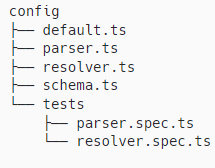
\includegraphics{file-tree/config-tree.png}
  \caption{File tree of files that implement the configuration system}
\end{figure}

The \texttt{defailt.ts} file contains the default configuration values that are used if no configuration file is found.

\begin{listing}[H]
  \tsfile{implementation/code/cli/config-default.ts}
  \caption{Contents of \texttt{default.ts} file}
\end{listing}

The \texttt{resolver.ts} file contains the logic that searches for configuration files and determinate the order in which they are to be loaded and merged.
To load a configuratation file \texttt{fromFile} static method from \texttt{HydraConfig} class is used. It takes a path to the configuration file and returns a \texttt{HydraConfig} instance.

\begin{listing}[H]
  \tsfile{implementation/code/cli/config-parser.ts}
  \caption{\texttt{parser.ts} file containing the \texttt{HydraConfig} class}
\end{listing}

The config file structure is validated using schema defined in \texttt{schema.ts} file.
To define and validate the schema \texttt{zod} library is used \cite{zod}.

\begin{listing}[H]
  \tsfile{implementation/code/cli/config-schema.ts}
  \caption{Config schema definition using \texttt{zod} library}
\end{listing}

The \texttt{HydraConfig} class is employed by both the \textbf{backend} and \textbf{cli} application to load configuration files.
If the \textbf{enable} flag under \textbf{socket} entry is set \textbf{true} then the unix socket is created and the \textbf{path} value is used as the path to the socket.
In contrast, when the \textbf{enable} flag is configured as \textbf{false}, the socket is not generated.
This absence of a socket results in a communication breakdown between the \textbf{cli} application and the \textbf{backend} application, effectively disabling this feature.

\begin{listing}[H]
  \yamlfile{implementation/code/cli/config-example.yml}
  \caption{Example hydra configuration file with enabled socket communication}
\end{listing}

\subsection{Socket creation and API definition}

The management api over unix socket is created upon application satrtup if feature is enabled in the configuration file.

\begin{listing}[H]
  \tsfile{implementation/code/cli/backend-init.ts}
  \caption{Backend initialization code}
\end{listing}

The management module exposes a signel controller which define two routes:

\begin{itemize}
  \item \textbf{accounts/create-admin-account} - creates account with admin privileges
  \item \textbf{accounts/create-standard-account} - creates standard account subjected to permission system
\end{itemize}

This controler does not use any authentication or authorization middleware, as it is not exposed to the internet and is only accessible by the \textbf{cli} application.


\end{document}